\PassOptionsToPackage{unicode=true}{hyperref} % options for packages loaded elsewhere
\PassOptionsToPackage{hyphens}{url}
%
\documentclass[
]{book}
\usepackage{lmodern}
\usepackage{amssymb,amsmath}
\usepackage{ifxetex,ifluatex}
\ifnum 0\ifxetex 1\fi\ifluatex 1\fi=0 % if pdftex
  \usepackage[T1]{fontenc}
  \usepackage[utf8]{inputenc}
  \usepackage{textcomp} % provides euro and other symbols
\else % if luatex or xelatex
  \usepackage{unicode-math}
  \defaultfontfeatures{Scale=MatchLowercase}
  \defaultfontfeatures[\rmfamily]{Ligatures=TeX,Scale=1}
\fi
% use upquote if available, for straight quotes in verbatim environments
\IfFileExists{upquote.sty}{\usepackage{upquote}}{}
\IfFileExists{microtype.sty}{% use microtype if available
  \usepackage[]{microtype}
  \UseMicrotypeSet[protrusion]{basicmath} % disable protrusion for tt fonts
}{}
\makeatletter
\@ifundefined{KOMAClassName}{% if non-KOMA class
  \IfFileExists{parskip.sty}{%
    \usepackage{parskip}
  }{% else
    \setlength{\parindent}{0pt}
    \setlength{\parskip}{6pt plus 2pt minus 1pt}}
}{% if KOMA class
  \KOMAoptions{parskip=half}}
\makeatother
\usepackage{xcolor}
\IfFileExists{xurl.sty}{\usepackage{xurl}}{} % add URL line breaks if available
\IfFileExists{bookmark.sty}{\usepackage{bookmark}}{\usepackage{hyperref}}
\hypersetup{
  pdftitle={xaringan: Delivering Presentation with R Markdown},
  pdfauthor={Emi Tanaka, Joseph Casillas, Eric Nantz, Yihui Xie},
  pdfborder={0 0 0},
  breaklinks=true}
\urlstyle{same}  % don't use monospace font for urls
\usepackage{color}
\usepackage{fancyvrb}
\newcommand{\VerbBar}{|}
\newcommand{\VERB}{\Verb[commandchars=\\\{\}]}
\DefineVerbatimEnvironment{Highlighting}{Verbatim}{commandchars=\\\{\}}
% Add ',fontsize=\small' for more characters per line
\usepackage{framed}
\definecolor{shadecolor}{RGB}{248,248,248}
\newenvironment{Shaded}{\begin{snugshade}}{\end{snugshade}}
\newcommand{\AlertTok}[1]{\textcolor[rgb]{0.33,0.33,0.33}{#1}}
\newcommand{\AnnotationTok}[1]{\textcolor[rgb]{0.37,0.37,0.37}{\textbf{\textit{#1}}}}
\newcommand{\AttributeTok}[1]{\textcolor[rgb]{0.61,0.61,0.61}{#1}}
\newcommand{\BaseNTok}[1]{\textcolor[rgb]{0.06,0.06,0.06}{#1}}
\newcommand{\BuiltInTok}[1]{#1}
\newcommand{\CharTok}[1]{\textcolor[rgb]{0.5,0.5,0.5}{#1}}
\newcommand{\CommentTok}[1]{\textcolor[rgb]{0.37,0.37,0.37}{\textit{#1}}}
\newcommand{\CommentVarTok}[1]{\textcolor[rgb]{0.37,0.37,0.37}{\textbf{\textit{#1}}}}
\newcommand{\ConstantTok}[1]{\textcolor[rgb]{0,0,0}{#1}}
\newcommand{\ControlFlowTok}[1]{\textcolor[rgb]{0.27,0.27,0.27}{\textbf{#1}}}
\newcommand{\DataTypeTok}[1]{\textcolor[rgb]{0.27,0.27,0.27}{#1}}
\newcommand{\DecValTok}[1]{\textcolor[rgb]{0.06,0.06,0.06}{#1}}
\newcommand{\DocumentationTok}[1]{\textcolor[rgb]{0.37,0.37,0.37}{\textbf{\textit{#1}}}}
\newcommand{\ErrorTok}[1]{\textcolor[rgb]{0.14,0.14,0.14}{\textbf{#1}}}
\newcommand{\ExtensionTok}[1]{#1}
\newcommand{\FloatTok}[1]{\textcolor[rgb]{0.06,0.06,0.06}{#1}}
\newcommand{\FunctionTok}[1]{\textcolor[rgb]{0,0,0}{#1}}
\newcommand{\ImportTok}[1]{#1}
\newcommand{\InformationTok}[1]{\textcolor[rgb]{0.37,0.37,0.37}{\textbf{\textit{#1}}}}
\newcommand{\KeywordTok}[1]{\textcolor[rgb]{0.27,0.27,0.27}{\textbf{#1}}}
\newcommand{\NormalTok}[1]{#1}
\newcommand{\OperatorTok}[1]{\textcolor[rgb]{0.43,0.43,0.43}{\textbf{#1}}}
\newcommand{\OtherTok}[1]{\textcolor[rgb]{0.37,0.37,0.37}{#1}}
\newcommand{\PreprocessorTok}[1]{\textcolor[rgb]{0.37,0.37,0.37}{\textit{#1}}}
\newcommand{\RegionMarkerTok}[1]{#1}
\newcommand{\SpecialCharTok}[1]{\textcolor[rgb]{0,0,0}{#1}}
\newcommand{\SpecialStringTok}[1]{\textcolor[rgb]{0.5,0.5,0.5}{#1}}
\newcommand{\StringTok}[1]{\textcolor[rgb]{0.5,0.5,0.5}{#1}}
\newcommand{\VariableTok}[1]{\textcolor[rgb]{0,0,0}{#1}}
\newcommand{\VerbatimStringTok}[1]{\textcolor[rgb]{0.5,0.5,0.5}{#1}}
\newcommand{\WarningTok}[1]{\textcolor[rgb]{0.37,0.37,0.37}{\textbf{\textit{#1}}}}
\usepackage{longtable,booktabs}
% Allow footnotes in longtable head/foot
\IfFileExists{footnotehyper.sty}{\usepackage{footnotehyper}}{\usepackage{footnote}}
\makesavenoteenv{longtable}
\usepackage{graphicx,grffile}
\makeatletter
\def\maxwidth{\ifdim\Gin@nat@width>\linewidth\linewidth\else\Gin@nat@width\fi}
\def\maxheight{\ifdim\Gin@nat@height>\textheight\textheight\else\Gin@nat@height\fi}
\makeatother
% Scale images if necessary, so that they will not overflow the page
% margins by default, and it is still possible to overwrite the defaults
% using explicit options in \includegraphics[width, height, ...]{}
\setkeys{Gin}{width=\maxwidth,height=\maxheight,keepaspectratio}
\setlength{\emergencystretch}{3em}  % prevent overfull lines
\providecommand{\tightlist}{%
  \setlength{\itemsep}{0pt}\setlength{\parskip}{0pt}}
\setcounter{secnumdepth}{5}
% Redefines (sub)paragraphs to behave more like sections
\ifx\paragraph\undefined\else
  \let\oldparagraph\paragraph
  \renewcommand{\paragraph}[1]{\oldparagraph{#1}\mbox{}}
\fi
\ifx\subparagraph\undefined\else
  \let\oldsubparagraph\subparagraph
  \renewcommand{\subparagraph}[1]{\oldsubparagraph{#1}\mbox{}}
\fi

% set default figure placement to htbp
\makeatletter
\def\fps@figure{htbp}
\makeatother

\usepackage{booktabs}
\usepackage{amsthm}
\makeatletter
\def\thm@space@setup{%
  \thm@preskip=8pt plus 2pt minus 4pt
  \thm@postskip=\thm@preskip
}
\makeatother
\usepackage[]{natbib}
\bibliographystyle{apalike}

\title{xaringan: Delivering Presentation with R Markdown}
\author{Emi Tanaka, Joseph Casillas, Eric Nantz, Yihui Xie}
\date{2019-03-09}

\begin{document}
\maketitle

{
\setcounter{tocdepth}{2}
\tableofcontents
}
\hypertarget{preface}{%
\chapter*{Preface}\label{preface}}


Hello.

\hypertarget{author}{%
\chapter*{About the Authors}\label{author}}


We are a team of shinobi and kunoichi who wish to share the fun and secrets of the \textbf{xaringan} package with you.

\hypertarget{emi-tanaka}{%
\section*{Emi Tanaka}\label{emi-tanaka}}


Lead author, and the ninja theme author.

\hypertarget{joseph-casillas}{%
\section*{Joseph Casillas}\label{joseph-casillas}}


Contributor of xaringan.

\hypertarget{eric-nantz}{%
\section*{Eric Nantz}\label{eric-nantz}}


Host of the R Podcast.

\hypertarget{yihui-xie}{%
\section*{Yihui Xie}\label{yihui-xie}}


Yihui Xie (\url{https://yihui.name}) is a software engineer at RStudio (\url{https://www.rstudio.com}). He earned his PhD from the Department of Statistics, Iowa State University. He is interested in interactive statistical graphics and statistical computing. As an active R user, he has authored several R packages, such as \textbf{knitr}, \textbf{bookdown}, \textbf{blogdown}, \textbf{xaringan}, \textbf{tinytex}, \textbf{animation}, \textbf{DT}, \textbf{tufte}, \textbf{formatR}, \textbf{fun}, \textbf{xfun}, \textbf{mime}, \textbf{highr}, \textbf{servr}, and \textbf{Rd2roxygen}, among which the \textbf{animation} package won the 2009 John M. Chambers Statistical Software Award (ASA). He also co-authored a few other R packages, including \textbf{shiny}, \textbf{rmarkdown}, and \textbf{leaflet}.

He has authored two books, \emph{Dynamic Documents with knitr} \citep{xie2015}, and \emph{bookdown: Authoring Books and Technical Documents with R Markdown} \citep{xie2016}, and co-authored the book, \emph{blogdown: Creating Websites with R Markdown} \citep{xie2017}.

In 2006, he founded the Capital of Statistics (\url{https://cosx.org}), which has grown into a large online community on statistics in China. He initiated the Chinese R conference in 2008, and has been involved in organizing R conferences in China since then. During his PhD training at Iowa State University, he won the Vince Sposito Statistical Computing Award (2011) and the Snedecor Award (2012) in the Department of Statistics.

He occasionally rants on Twitter (\url{https://twitter.com/xieyihui}, well not so much these days), and most of the time you can find him on GitHub (\url{https://github.com/yihui}).

He enjoys spicy food as much as classical Chinese literature and is a master hacker freeing the frustation of thousands of people that would have needed to repeatedly copy-and-paste the R output and saving science with the gift of reproducible research.

\hypertarget{intro}{%
\chapter{Introduction}\label{intro}}

In late 2016, Yihui discovered remark.js (Bang 2018) and loved it at the first sight. A few weeks later in the R Markdown ecosystem (Allaire et al.~2018), an R package was born and named xaringan (???), which nobody knows how to pronounce (including Yihui himself, because it was adapted from the Japanese manga series Naruto by Kishimoto (2007)). Anyway, this package has gained some popularity, and some CSS ninja have started contributing themes to it. One day, Yihui was thinking about creating a gallery for existing themes in xaringan. After a few replies in the \href{https://github.com/yihui/xaringan/issues/172\#issuecomment-434065692}{Github issue}, he realized there might be enough topics on xaringan for a short book. Accidentally, he invented a new development model for writing books: the Github-issue-driven book development.

Ideas so far:

This could include the basics:

\begin{itemize}
\tightlist
\item
  Installation
\item
  Motivation - Why slideshows using R Markdown (should mention about ioslides too and differences to it)
\item
  Structure of the book
\item
  etc
\end{itemize}

\hypertarget{basics}{%
\chapter{Basics}\label{basics}}

In this chapter you will get up and moving with your first HTML presentation using \texttt{xaringan}. Specifically, we will cover the basics regarding getting started and generating your HTML slides, as well as talk about some markdown and \texttt{xaringan}-specific syntax considerations. Next, you will learn how to incorporate some light customization to give your slides a more personal touch. This chapter concludes with some examples of best practices for including R code in your \texttt{xaringan} presentations.

\hypertarget{getting-started}{%
\section{Getting started}\label{getting-started}}

Before we get started you must install the \texttt{xaringan} package if you have not already done so. You can install \texttt{xaringan} via CRAN by typing \texttt{install.packages("xaringan")} into the console. If you use the RStudio IDE, you can install \texttt{xaringan} by clicking the packages tab and searching for \texttt{xaringan}. If you prefer to be on the cutting edge of software development you can install the latest version of \texttt{xaringan} directly from github by typing \texttt{devtools::install\_github("yihui/xaringan")} into the console, but note that this method requires that you have \texttt{devtools} installed first.

Once you have installed \texttt{xaringan} you are ready to get started. We will begin with the simplified template that is provided in the \texttt{xaringan} package. This will allow you to learn the basics of \texttt{xaringan} quickly and provide you with easy access to an example that you can refer back to if necessary. You can create a new copy of the template using the menu in the RStudio IDE. Click ``File'' → ``New File'' → ``R Markdown'' → ``From Template'' → ``Ninja Presentation''.\footnote{If you are not using RStudio, that's fine too. HTML presentations generated using \texttt{xaringan} are just standard R Markdown (.Rmd) files, so you can create one from scratch using your text editor of choice and follow the examples all the same.} Once you click ``OK'' a new .Rmd file will automatically open in RStudio.

\hypertarget{front-matter}{%
\subsection{Front matter}\label{front-matter}}

As touched upon above, \texttt{xaringan} slides are generated from R Markdown files. This means that your presentation will have YAML front matter, like any other .Rmd file.\footnote{You can learn the basics of R Markdown here: \url{https://rmarkdown.rstudio.com/lesson-1.html}} Below is the front matter of our template. If you are not using the RStudio IDE, feel free to copy the front matter and paste it into your .Rmd document.

\begin{Shaded}
\begin{Highlighting}[]
\OperatorTok{---}
\NormalTok{title}\OperatorTok{:}\StringTok{ "Presentation Ninja"}
\NormalTok{subtitle}\OperatorTok{:}\StringTok{ "⚔<br/>with xaringan"}
\NormalTok{author}\OperatorTok{:}\StringTok{ "Yihui Xie"}
\NormalTok{date}\OperatorTok{:}\StringTok{ "2016/12/12 (updated: `r Sys.Date()`)"}
\NormalTok{output}\OperatorTok{:}
\StringTok{  }\NormalTok{xaringan}\OperatorTok{::}\NormalTok{moon_reader}\OperatorTok{:}
\StringTok{    }\NormalTok{lib_dir}\OperatorTok{:}\StringTok{ }\NormalTok{libs}
\NormalTok{    nature}\OperatorTok{:}
\StringTok{      }\NormalTok{highlightStyle}\OperatorTok{:}\StringTok{ }\NormalTok{github}
\NormalTok{      highlightLines}\OperatorTok{:}\StringTok{ }\NormalTok{true}
\NormalTok{      countIncrementalSlides}\OperatorTok{:}\StringTok{ }\NormalTok{false}
\OperatorTok{---}
\end{Highlighting}
\end{Shaded}

Here you can include all of the importnat information you would typically include in the title slide of your presentation. The main difference between HTML slides generated in \texttt{xaringan} and any other R Markdown file is that the HTML output is generated using the output format \texttt{moon\_reader}. The output format serves as a wrapper for remark.js, which is doing all of the heavy lifting under the hood. This information may not seem too important to most people, but it is worth mentioning because the \texttt{moon\_reader} format is the only part of the front matter that is truly necessary to create your slides. In fact, if you were feeling adventurous you could create slides that \emph{only} contained this information, i.e., \texttt{output:\ xaringan::moon\_reader}, and delete all the other information. We will come back to remark.js in chapter 6, Advanced Topics. Now you are ready to generate your first HTML slides using \texttt{xaringan}.

\hypertarget{generating-your-slides}{%
\subsection{Generating your slides}\label{generating-your-slides}}

There are several methods for generating and working with slides in a \texttt{xaringan} presentation, which we will now cover. First things first, save your .Rmd file to a location on your hard drive and give your presentation file a name. If you are using RStudio, simply click the \texttt{Knit} button at the top of the application window and you will be prompted to save the .Rmd file. RStudio will render the slides after you save and they will automatically appear in the Viewer window. \textbf{Pro tip}: you can install the \texttt{infinite\_moon\_reader} RStudio Addin which will allow you to update your slides in real time (more on this in Chapter 6). If you are not using RStudio, save your .Rmd file and then you can generate your slides from the console by typing \texttt{rmarkdown::render("your-file-name.Rmd")}.

\hypertarget{exploring-a-xaringan-presentation}{%
\subsection{\texorpdfstring{Exploring a \texttt{xaringan} presentation}{Exploring a xaringan presentation}}\label{exploring-a-xaringan-presentation}}

Before we go into the details of customizing your slides, let's explore the \texttt{xaringan} presentaion we just created. If you are using RStudio the presentation should have opened automatically in the Viewer panel. If you rendered your slides manually, double click the HTML file that was produced to open it in your web browser of choice.\footnote{Note: if you are creating your slides manually, your presentation will not have much content yet. You can explore the same example slides here: \url{https://slides.yihui.name/xaringan/}} You should see something like this:

\begin{figure}
\centering

\includegraphics{img/02_title-slide.png}
\caption{title\_slide}
\end{figure}

Use the left and right arrow keys to navigate the slides. There are a whole host of features at your finger tips, but we will only highlight two for now. You can type the number of a given slide and press the ``enter''/``return'' key to navigate to that slide, i.e., ``9'' + ``return''. If you press the ``p'' key you will enter ``Presenter mode''. Cool, right? You can press the ``p'' key again to leave presenter mode. Type the ``h'' key to see a list of some of the other features. As mentioned, we will talk more about these in Chapter 6. In the next section we will cover the basics for editing your \texttt{xaringan} presentation.

\hypertarget{editing-your-slides}{%
\section{Editing your slides}\label{editing-your-slides}}

Editing a \texttt{xaringan} presentation is quite simple. If you are already familiar with Markdown syntax, you will be a \texttt{xaringan} ninja with little effort. If you are new to Markdown syntax you can cover the basics at \url{https://rmarkdown.rstudio.com/lesson-8.html}. For now, let's start with a clean slate and delete everything in our template \textbf{after} the YAML front matter. That is, delete everything in your file \textbf{after} line 13.

\hypertarget{general-syntax}{%
\subsection{General syntax}\label{general-syntax}}

\texttt{xaringan} shares all of the basic features of Markdown syntax. This means you can create \textbf{bold} text and \emph{italics} by surrounding text with double or single stars, i.e., **bold** and *italics*, respectively. You can also create unordered lists:

\begin{itemize}
\tightlist
\item
  this
\item
  is
\item
  and unordered list
\end{itemize}

and ordered lists:

\begin{enumerate}
\def\labelenumi{\arabic{enumi}.}
\tightlist
\item
  This is 1
\item
  This is 2
\item
  This is 3
\end{enumerate}

like so:

\begin{Shaded}
\begin{Highlighting}[]
\NormalTok{You can also create unordered lists}\OperatorTok{:}\StringTok{ }

\OperatorTok{-}\StringTok{ }\NormalTok{this }
\OperatorTok{-}\StringTok{ }\NormalTok{is }
\OperatorTok{-}\StringTok{ }\NormalTok{and unordered list}

\NormalTok{and ordered lists}\OperatorTok{:}\StringTok{ }

\FloatTok{1.}\NormalTok{ This is }\DecValTok{1}
\FloatTok{2.}\NormalTok{ This is }\DecValTok{2}
\FloatTok{3.}\NormalTok{ This is }\DecValTok{3}
\end{Highlighting}
\end{Shaded}

We won't cover all of the details of Markdown syntax here, but rather highlight some of the \texttt{xaringan}-specific features.

\hypertarget{creating-individual-slides}{%
\subsection{Creating individual slides}\label{creating-individual-slides}}

In \texttt{xaringan} you use a sequence of three hyphens, \texttt{-\/-\/-}, to separate slides.\footnote{Note that this is slightly different from ioSlides where hastags, \#\#, are used to dilineate where a new slide begins.} You are not required to include any headers, but you can using standard Markdown syntax, i.e., hashtags. Thus, we could create a simple slide including a header, a subsection, and a list by including the following code after the YAML front matter:\footnote{This implies that the final three hyphens of the YAML front matter indicate the end of the title slide and the beginning of slide \#2.}

\begin{Shaded}
\begin{Highlighting}[]
\CommentTok{# What I do on the weekends}

\CommentTok{## Hobbies}

\OperatorTok{-}\StringTok{ }\NormalTok{Run }\ControlFlowTok{in}\NormalTok{ the park}
\OperatorTok{-}\StringTok{ }\NormalTok{Walk my dogs}
\OperatorTok{-}\StringTok{ }\NormalTok{Create presentations }\ControlFlowTok{in} \StringTok{`}\DataTypeTok{xaringan}\StringTok{`}
\end{Highlighting}
\end{Shaded}

Feel free to copy this into your file and click ``Knit''. The output should render like this:

\begin{figure}
\centering
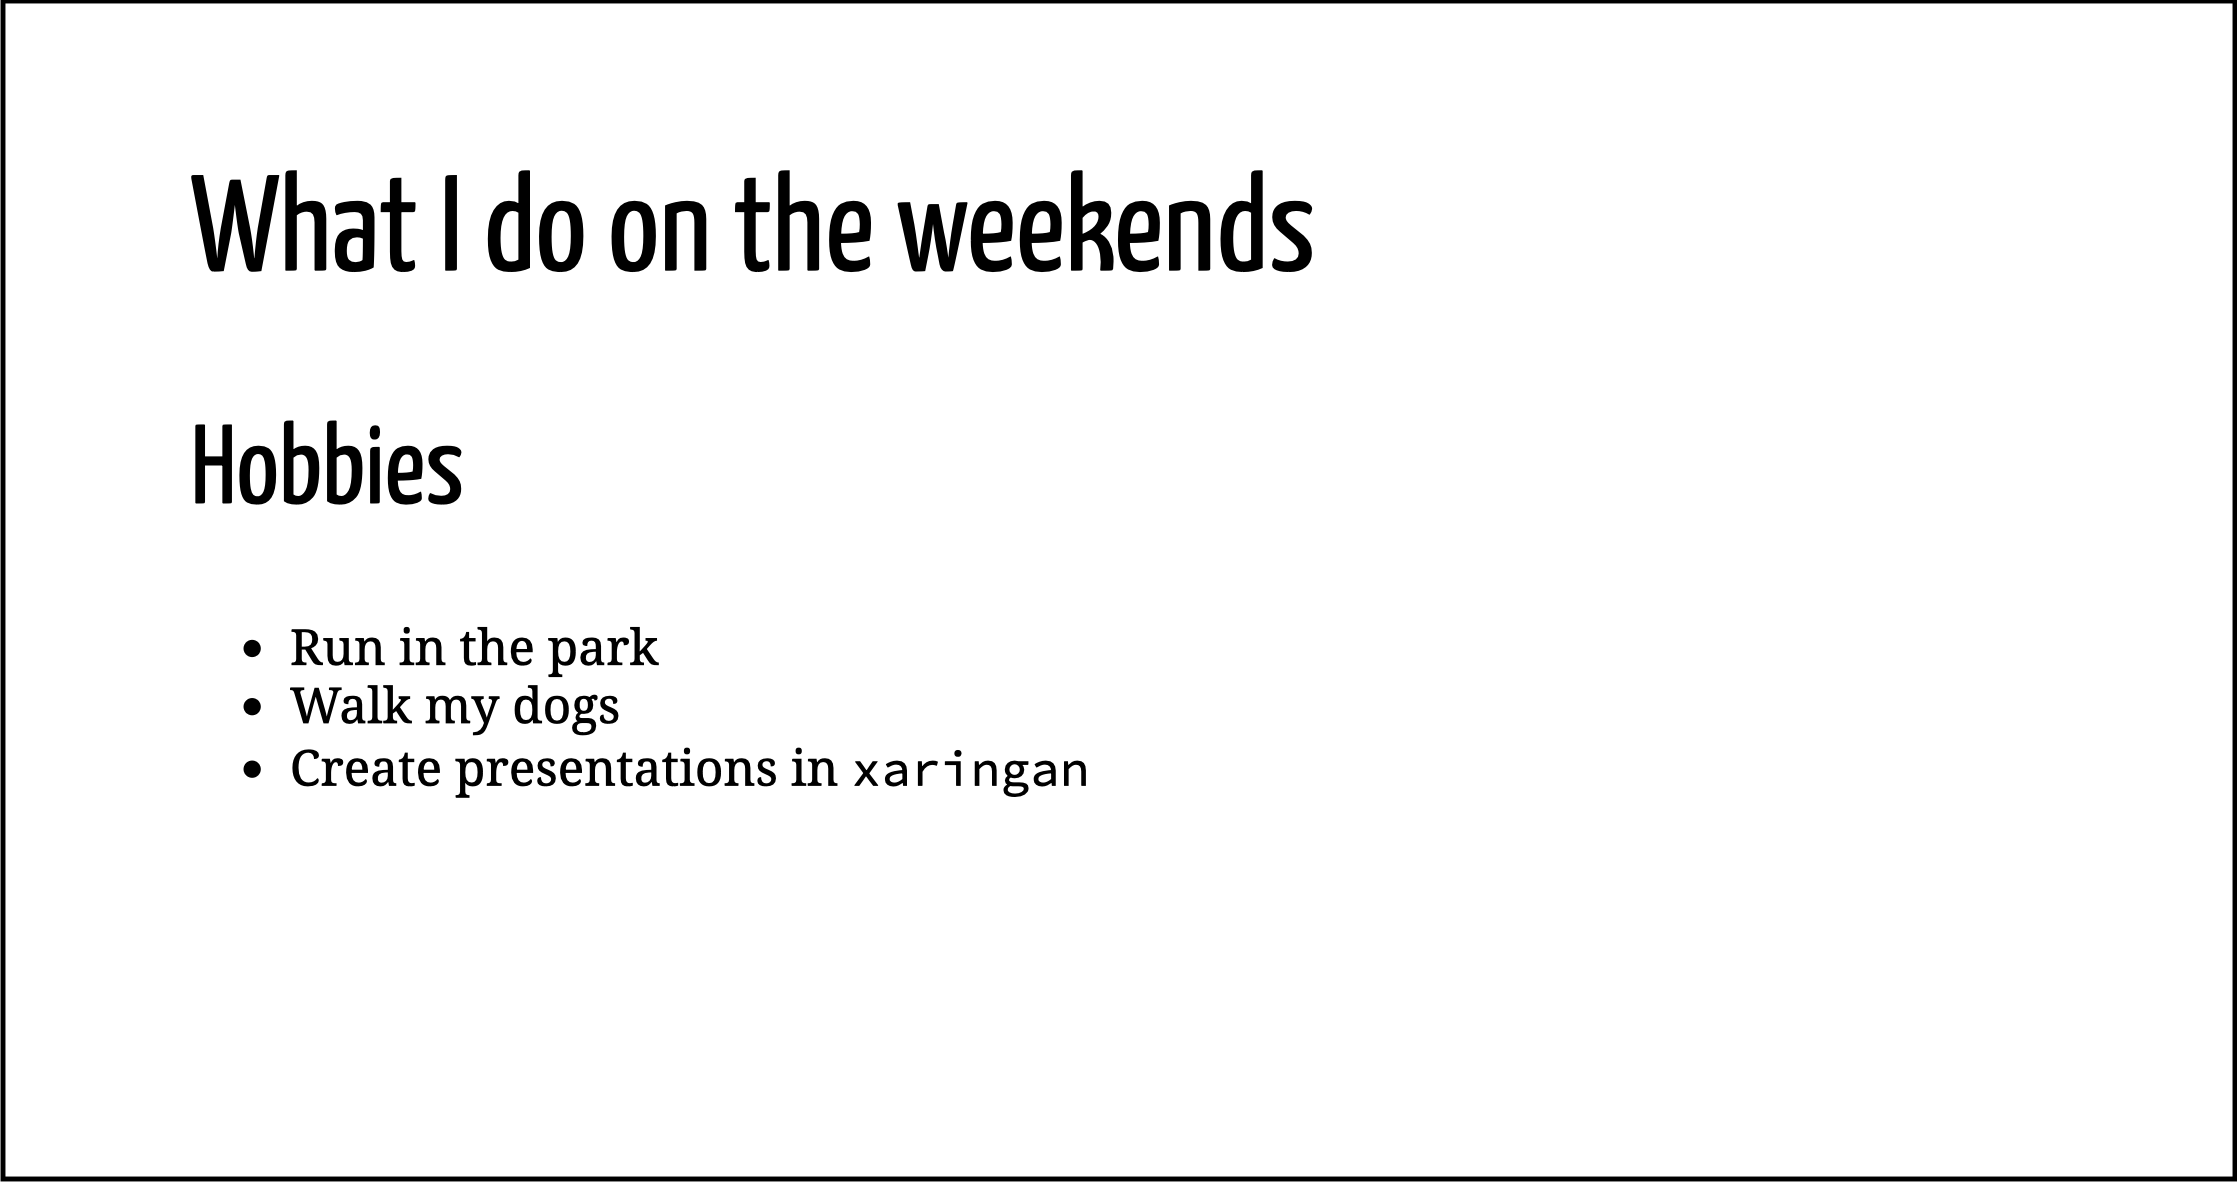
\includegraphics{img/02_basics-slide-example.png}
\caption{basics-slide-example}
\end{figure}

\hypertarget{incremental-slides}{%
\subsection{Incremental slides}\label{incremental-slides}}

It is often useful in a presentation to incrementally show information. This is easily done in \texttt{xaringan} using two hyphens, \texttt{-\/-}. Careful, don't confuse this with the three hyphen slide breaks! You can incrementally reveal pretty much any type of inforamtion you put into a slide. Let's add some examples to our presentation by creating a new slide. Don't forget, to create the new slide we need to add \texttt{-\/-\/-}. In our case, this would be after the last line of list we created in the previous example. For the sake of completeness I will include the code from both slides below.

\begin{Shaded}
\begin{Highlighting}[]
\CommentTok{# What I do on the weekends}

\CommentTok{## Hobbies}

\OperatorTok{-}\StringTok{ }\NormalTok{Run }\ControlFlowTok{in}\NormalTok{ the park}
\OperatorTok{-}\StringTok{ }\NormalTok{Walk my dogs}
\OperatorTok{-}\StringTok{ }\NormalTok{Create presentations }\ControlFlowTok{in} \StringTok{`}\DataTypeTok{xaringan}\StringTok{`}

\OperatorTok{---}

\CommentTok{# Incremental slides}

\CommentTok{### Sentence example}

\NormalTok{This sentence}
\OperatorTok{--}
\NormalTok{is displayed }
\OperatorTok{--}
\NormalTok{incrementally. }
\end{Highlighting}
\end{Shaded}

If you copy this example and Knit your slides you will notice notice that the sentence is rendered incrementally on a single line even though it is written in on separate lines. This is because the double hyphen, \texttt{-\/-}, has to be on its own line with no spaces before or after in order to work properly. We can also use this technique to reveal items of a list incrementally:

\begin{Shaded}
\begin{Highlighting}[]
\CommentTok{# Incremental slides}

\CommentTok{### Non-incremental sentence example}

\NormalTok{This sentence is no longer displayed incrementally. }

\CommentTok{### Incremental list example}

\OperatorTok{-}\StringTok{ }\NormalTok{An incremental list}
\OperatorTok{--}

\OperatorTok{-}\StringTok{ }\NormalTok{Is useful}
\OperatorTok{--}

\OperatorTok{-}\StringTok{ }\NormalTok{Sometimes}
\end{Highlighting}
\end{Shaded}

\hypertarget{multi-column-slides}{%
\subsection{Multi-column slides}\label{multi-column-slides}}

Another common feature of presentations is to display content in two columns. This is easibly acheived in \texttt{xaringan} using a bit of remark.js syntax. You will recognize the remark.js syntax because it begins with a period and and opening bracket, \texttt{.{[}}, and end with a closing bracket, \texttt{{]}}. Specifically, there are two options for creating two-column layouts. The first option is to use \texttt{.left-column{[}{]}} and \texttt{.right-column{[}{]}}. For example:

\begin{Shaded}
\begin{Highlighting}[]
\CommentTok{# Two column slides}

\NormalTok{.left}\OperatorTok{-}\NormalTok{column[}
\NormalTok{Left column information here.}
\NormalTok{]}

\NormalTok{.right}\OperatorTok{-}\NormalTok{column[}
\NormalTok{Right column information here.}
\NormalTok{]}
\end{Highlighting}
\end{Shaded}

would render like this:

\begin{figure}
\centering
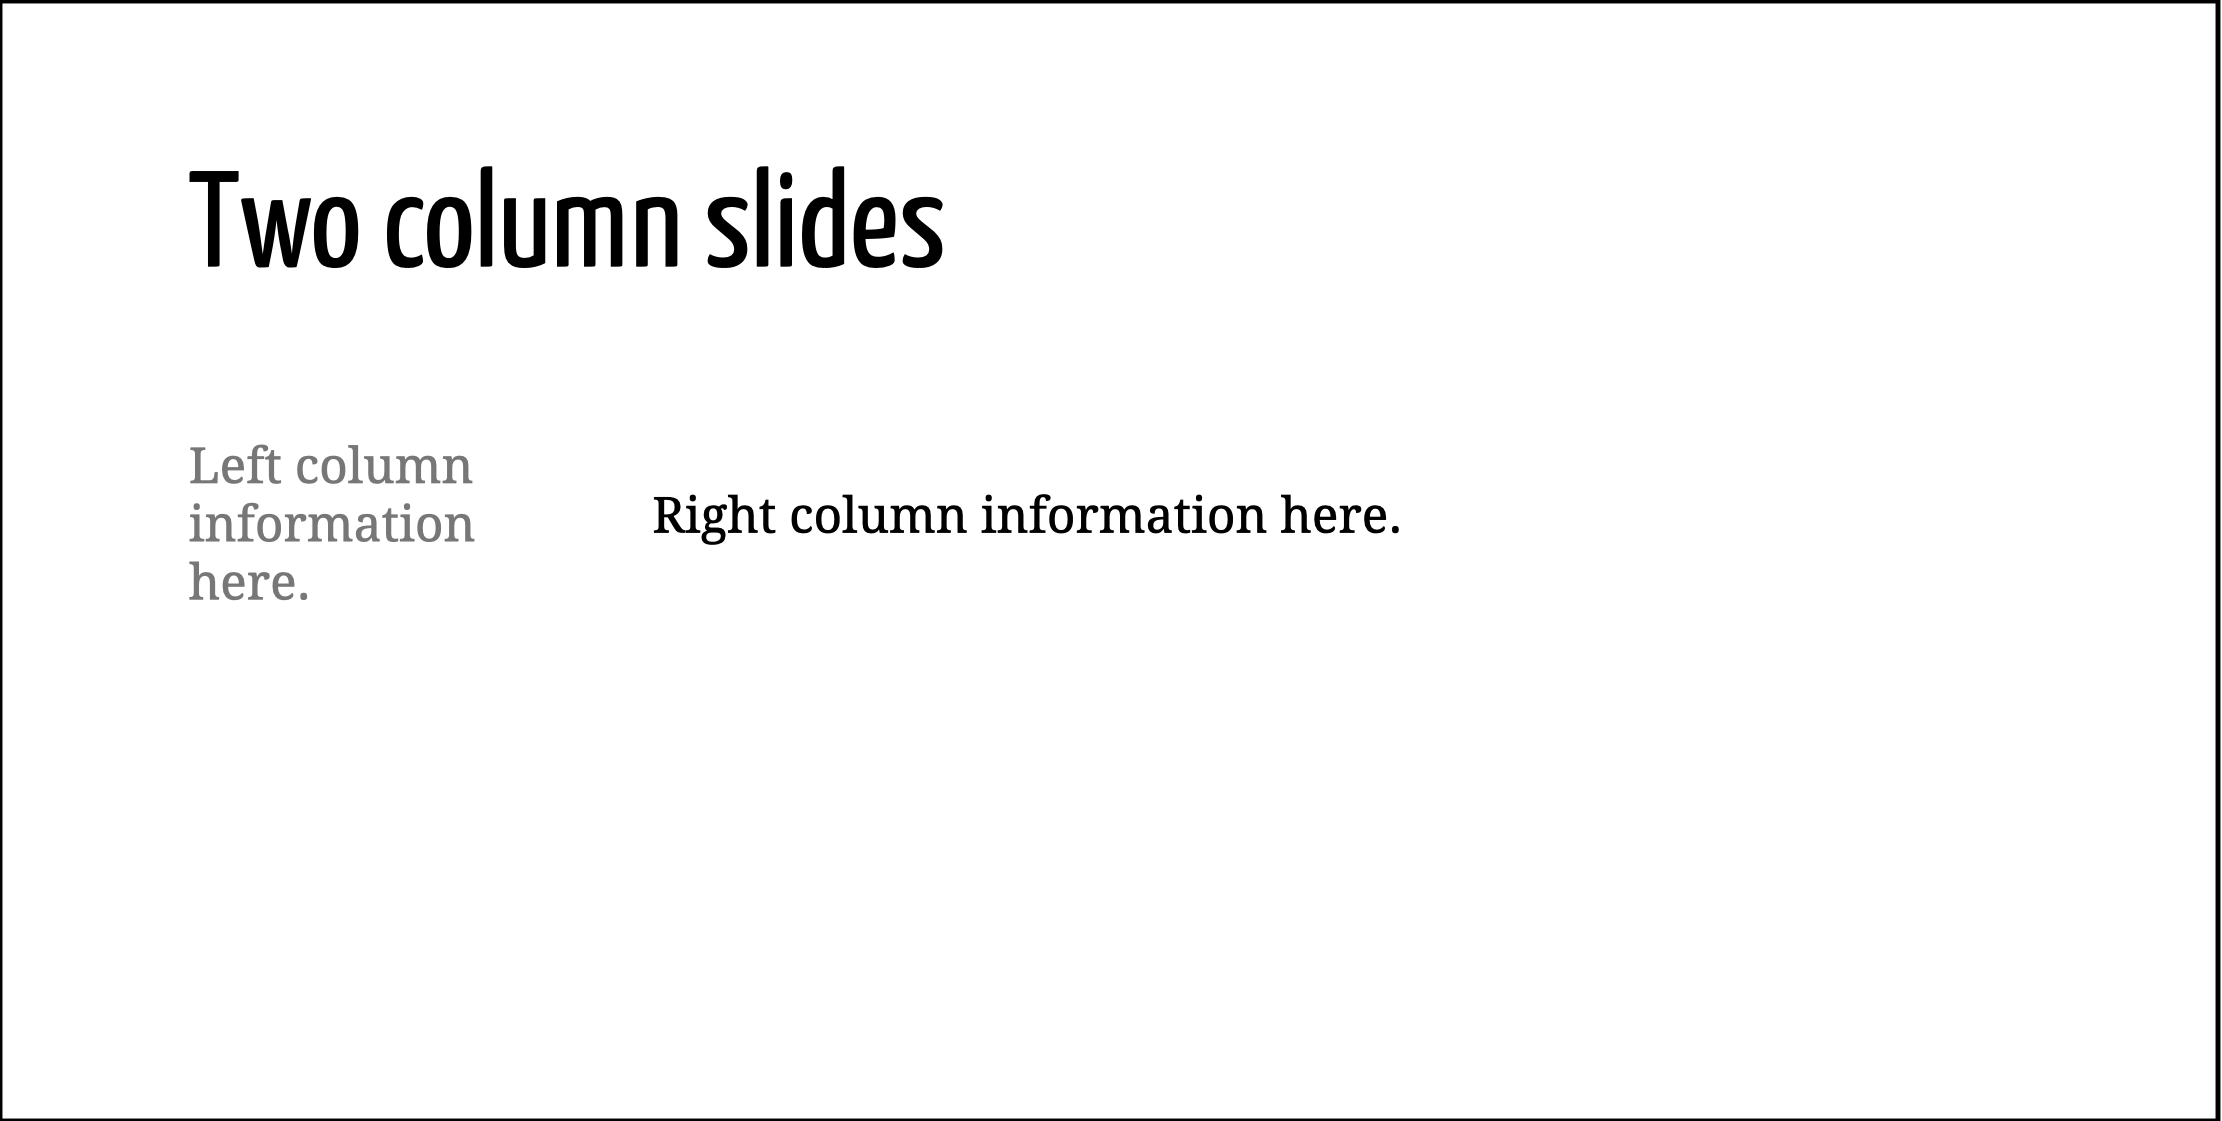
\includegraphics{img/02_basics-two-column_1.png}
\caption{basic-two-column-1}
\end{figure}

As you can see, this divides the left column into approxametely 1/3 of the slide width and the right column contains the remaining 2/3. This may be most useful when you need show a list on one side and need more space for content on the other. Another option is to divide the slide equally down the middle. You can achieve this by using \texttt{.pull-left{[}{]}} and \texttt{.pull-right{[}{]}}. For example:

\begin{Shaded}
\begin{Highlighting}[]
\CommentTok{# Two columns slides (cont.)}

\NormalTok{.pull}\OperatorTok{-}\NormalTok{left[}
\NormalTok{Left column information here.}
\NormalTok{]}

\NormalTok{.pull}\OperatorTok{-}\NormalTok{right[}
\NormalTok{Right column information here}
\NormalTok{]}
\end{Highlighting}
\end{Shaded}

\begin{figure}
\centering
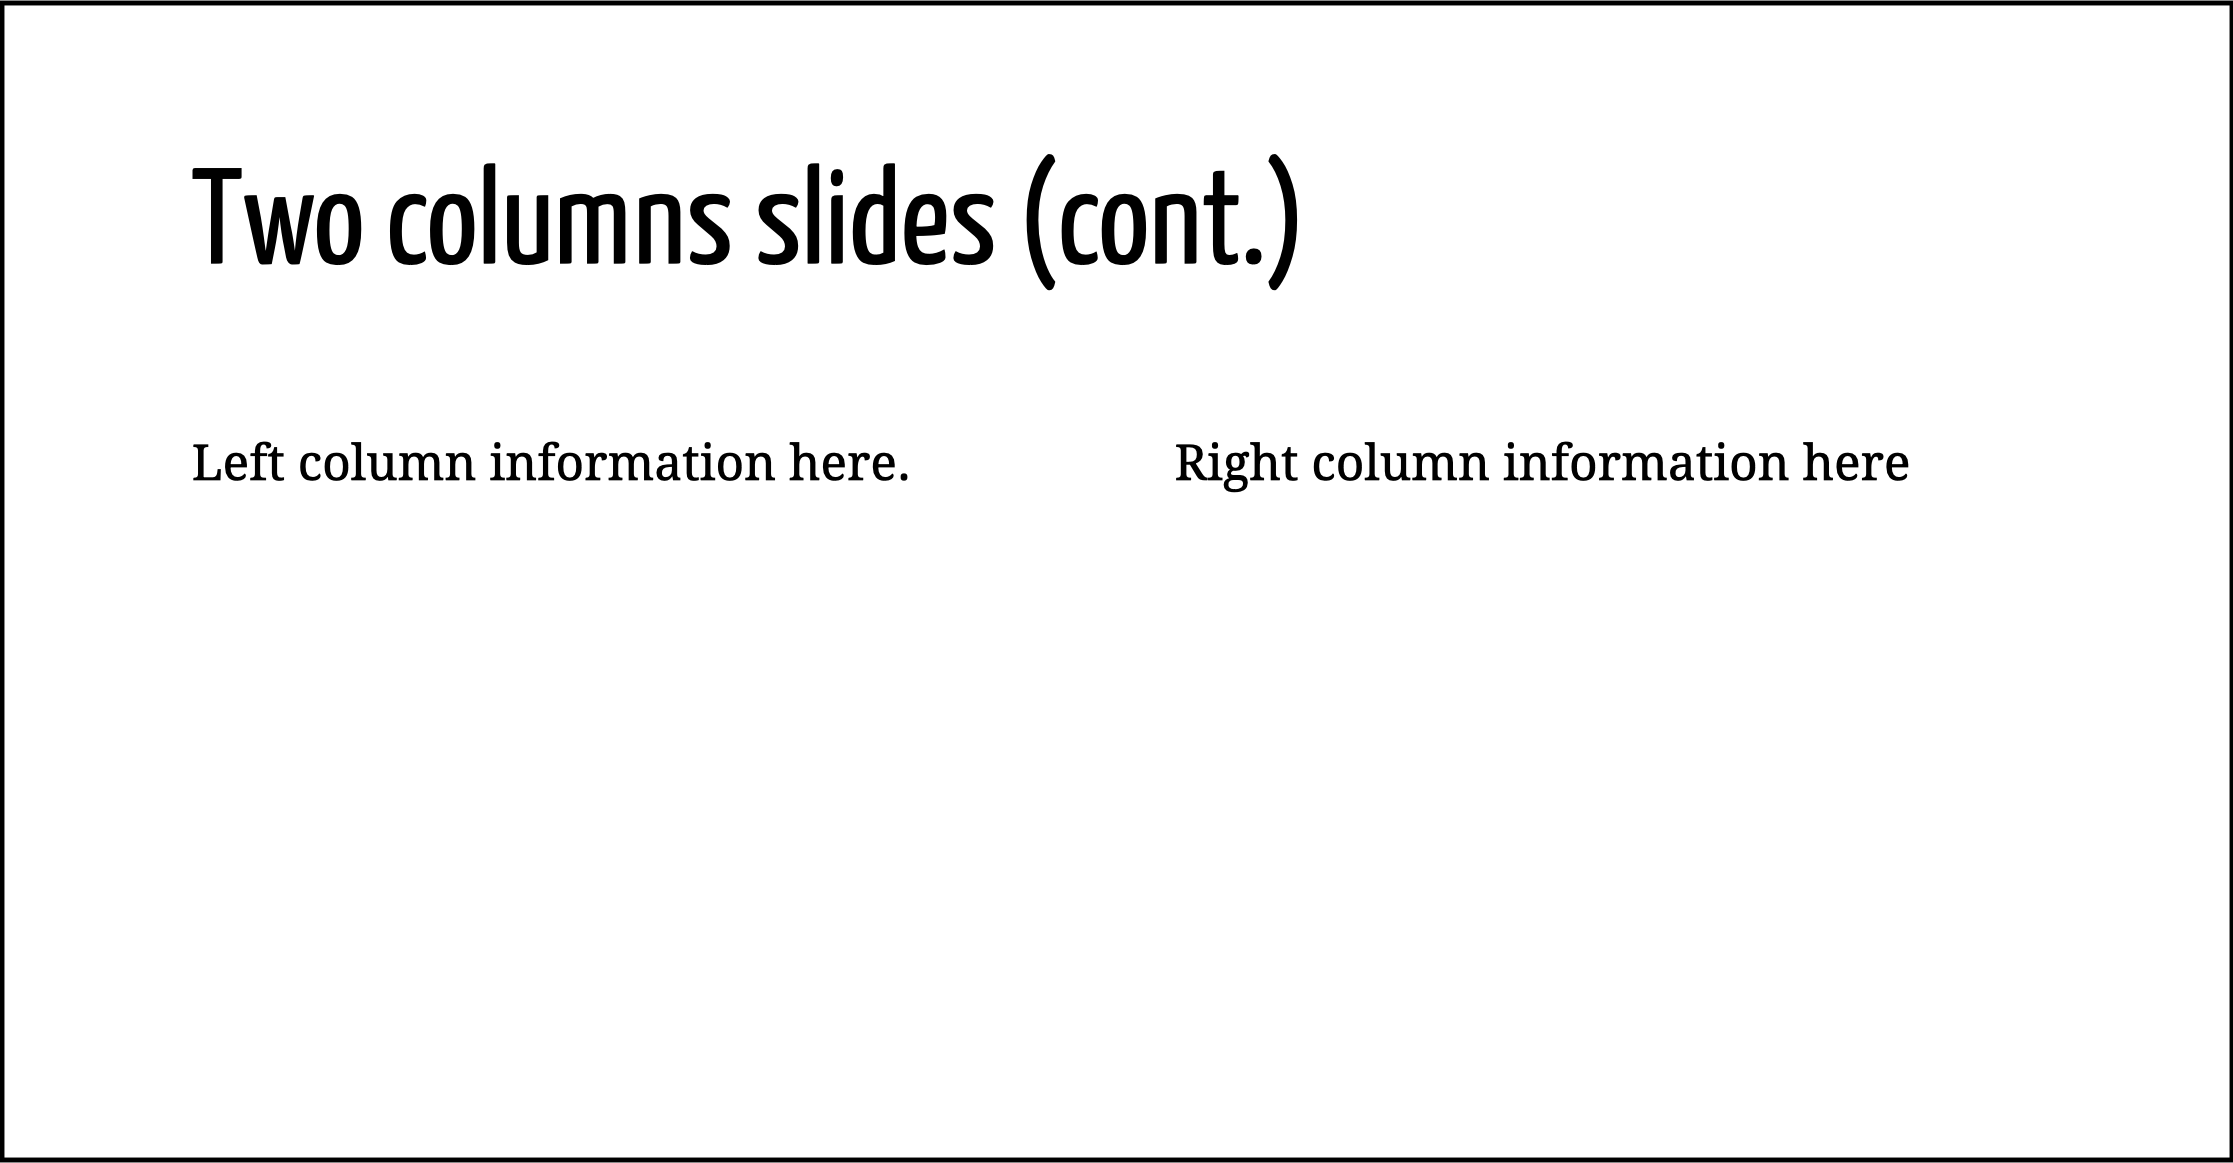
\includegraphics{img/02_basics-two-column_2.png}
\caption{basic-two-column-2}
\end{figure}

\hypertarget{math}{%
\subsection{math}\label{math}}

\hypertarget{making-it-yours}{%
\section{Making it yours}\label{making-it-yours}}

\hypertarget{images-gifs}{%
\subsection{Images, gifs}\label{images-gifs}}

\begin{itemize}
\tightlist
\item
  knitr
\item
  background images
\end{itemize}

\hypertarget{templates}{%
\subsection{Templates}\label{templates}}

\begin{itemize}
\tightlist
\item
  names(xaringan:::list\_css())
\end{itemize}

\hypertarget{htmlcssjs-basics}{%
\subsection{HTML/CSS/JS basics}\label{htmlcssjs-basics}}

\begin{itemize}
\tightlist
\item
  iframes

  \begin{itemize}
  \tightlist
  \item
    include other websites, shiny apps
  \end{itemize}
\item
  basic customization (CSS, JS)

  \begin{itemize}
  \tightlist
  \item
    colors, counters, tweets
  \end{itemize}
\end{itemize}

\hypertarget{incorporating-r-code}{%
\section{Incorporating R code}\label{incorporating-r-code}}

\begin{itemize}
\tightlist
\item
  analyses, plots and tables (some html widgets)
\item
  inline
\item
  knitr chunks
\item
  code highlighting (\texttt{*}, \texttt{\{\{\}\}}, and \texttt{\#\textless{}\textless{}}; \texttt{highlight.output})
\end{itemize}

\hypertarget{summary}{%
\section{Summary}\label{summary}}

\hypertarget{remarkjs}{%
\chapter{remark.js}\label{remarkjs}}

Ideas so far:

Features of the remark.js. Can draw out from wiki: \url{https://github.com/gnab/remark/wiki}

\hypertarget{feature}{%
\chapter{Features}\label{feature}}

Ideas so far:

\begin{itemize}
\tightlist
\item
  \texttt{xaringan} specific features not in remark.js
\end{itemize}

\hypertarget{publishing}{%
\chapter{Publishing}\label{publishing}}

Ideas so far:

\begin{itemize}
\tightlist
\item
  Where to host (netlify and github pages)
\item
  Offline
\item
  Any chance that RPubs to support xaringan in the future? Nice if tag feature is added to RPubs too. Or connect to some blogdown site with something similar to \url{https://www.overleaf.com/latex/templates}
\end{itemize}

\hypertarget{advanced}{%
\chapter{Advanced Topics}\label{advanced}}

So advanced that you need to train for weeks to know what it is.

\hypertarget{ideas}{%
\chapter{Ideas}\label{ideas}}

Some inspirations and theme showcase?

  \bibliography{book.bib,packages.bib}

\backmatter
\printindex

\end{document}
